\documentclass[twoside]{book}

% Packages required by doxygen
\usepackage{calc}
\usepackage{doxygen}
\usepackage{graphicx}
\usepackage[utf8]{inputenc}
\usepackage{makeidx}
\usepackage{multicol}
\usepackage{multirow}
\usepackage{fixltx2e}
\PassOptionsToPackage{warn}{textcomp}
\usepackage{textcomp}
\usepackage[nointegrals]{wasysym}
\usepackage[table]{xcolor}

% Font selection
\usepackage[T1]{fontenc}
\usepackage{mathptmx}
\usepackage[scaled=.90]{helvet}
\usepackage{courier}
\usepackage{amssymb}
\usepackage{sectsty}
\renewcommand{\familydefault}{\sfdefault}
\allsectionsfont{%
  \fontseries{bc}\selectfont%
  \color{darkgray}%
}
\renewcommand{\DoxyLabelFont}{%
  \fontseries{bc}\selectfont%
  \color{darkgray}%
}
\newcommand{\+}{\discretionary{\mbox{\scriptsize$\hookleftarrow$}}{}{}}

% Page & text layout
\usepackage{geometry}
\geometry{%
  a4paper,%
  top=2.5cm,%
  bottom=2.5cm,%
  left=2.5cm,%
  right=2.5cm%
}
\tolerance=750
\hfuzz=15pt
\hbadness=750
\setlength{\emergencystretch}{15pt}
\setlength{\parindent}{0cm}
\setlength{\parskip}{0.2cm}
\makeatletter
\renewcommand{\paragraph}{%
  \@startsection{paragraph}{4}{0ex}{-1.0ex}{1.0ex}{%
    \normalfont\normalsize\bfseries\SS@parafont%
  }%
}
\renewcommand{\subparagraph}{%
  \@startsection{subparagraph}{5}{0ex}{-1.0ex}{1.0ex}{%
    \normalfont\normalsize\bfseries\SS@subparafont%
  }%
}
\makeatother

% Headers & footers
\usepackage{fancyhdr}
\pagestyle{fancyplain}
\fancyhead[LE]{\fancyplain{}{\bfseries\thepage}}
\fancyhead[CE]{\fancyplain{}{}}
\fancyhead[RE]{\fancyplain{}{\bfseries\leftmark}}
\fancyhead[LO]{\fancyplain{}{\bfseries\rightmark}}
\fancyhead[CO]{\fancyplain{}{}}
\fancyhead[RO]{\fancyplain{}{\bfseries\thepage}}
\fancyfoot[LE]{\fancyplain{}{}}
\fancyfoot[CE]{\fancyplain{}{}}
\fancyfoot[RE]{\fancyplain{}{\bfseries\scriptsize Generated on Wed Jul 23 2014 10\+:00\+:21 for Progeny by Doxygen }}
\fancyfoot[LO]{\fancyplain{}{\bfseries\scriptsize Generated on Wed Jul 23 2014 10\+:00\+:21 for Progeny by Doxygen }}
\fancyfoot[CO]{\fancyplain{}{}}
\fancyfoot[RO]{\fancyplain{}{}}
\renewcommand{\footrulewidth}{0.4pt}
\renewcommand{\chaptermark}[1]{%
  \markboth{#1}{}%
}
\renewcommand{\sectionmark}[1]{%
  \markright{\thesection\ #1}%
}

% Indices & bibliography
\usepackage{natbib}
\usepackage[titles]{tocloft}
\setcounter{tocdepth}{3}
\setcounter{secnumdepth}{5}
\makeindex

% Hyperlinks (required, but should be loaded last)
\usepackage{ifpdf}
\ifpdf
  \usepackage[pdftex,pagebackref=true]{hyperref}
\else
  \usepackage[ps2pdf,pagebackref=true]{hyperref}
\fi
\hypersetup{%
  colorlinks=true,%
  linkcolor=blue,%
  citecolor=blue,%
  unicode%
}

% Custom commands
\newcommand{\clearemptydoublepage}{%
  \newpage{\pagestyle{empty}\cleardoublepage}%
}


%===== C O N T E N T S =====

\begin{document}

% Titlepage & ToC
\hypersetup{pageanchor=false,
             bookmarks=true,
             bookmarksnumbered=true,
             pdfencoding=unicode
            }
\pagenumbering{roman}
\begin{titlepage}
\vspace*{7cm}
\begin{center}%
{\Large Progeny \\[1ex]\large 1.\+0 }\\
\vspace*{1cm}
{\large Generated by Doxygen 1.8.7}\\
\vspace*{0.5cm}
{\small Wed Jul 23 2014 10:00:21}\\
\end{center}
\end{titlepage}
\clearemptydoublepage
\tableofcontents
\clearemptydoublepage
\pagenumbering{arabic}
\hypersetup{pageanchor=true}

%--- Begin generated contents ---
\chapter{Progeny Documentation}
\label{index}\hypertarget{index}{}\begin{DoxyAuthor}{Author}
Boris Bulanek  National Radiation Protection Institute, Bartoskova 28, 140 00, Praha 4  \href{mailto:boris.bulanek@suro.cz}{\tt boris.\-bulanek@suro.\-cz}  00420 226 518 279 
\end{DoxyAuthor}
\begin{DoxyDate}{Date}
02/19/13
\end{DoxyDate}
\hypertarget{index_about}{}\section{About the program}\label{index_about}
Program Progeny is created in order to provide simple and fast radon progeny concentration estimation.

Program allow user to obtain and store data using \href{http://www.sqlite.org}{\tt Sqlite} database.

The program uses some additional packages\-:
\begin{DoxyItemize}
\item U\-I (User Interface) framework \href{http://qt-project.org/}{\tt Qt}
\item a package for minimization \href{http://www.gnu.org/software/gsl/}{\tt G\-S\-L}
\item collection of {\ttfamily C++} tools \href{http://www.boost.org/}{\tt Boost}
\item database software called \href{http://www.sqlite.org}{\tt Sqlite}
\end{DoxyItemize}\hypertarget{index_Installation}{}\section{Installation}\label{index_Installation}
A single executable file {\bfseries progeny.\-exe} is created for Windows (7 or X\-P) users using \href{http://pic.dhe.ibm.com/infocenter/aix/v7r1/index.jsp?topic=%2Fcom.ibm.aix.prftungd%2Fdoc%2Fprftungd%2Fwhen_dyn_linking_static_linking.htm}{\tt static linking}. Linux users can execute {\ttfamily progeny.\-exe} using program \href{http://www.winehq.org/}{\tt wine}. I haven't tried to install the program on Mac but I believe that the installation is similar to installation on Linux. \hypertarget{index_Linux}{}\subsection{Linux}\label{index_Linux}
All of needed packages have to be in official repositories of your distribution as all of them are open source programs. For example in case of \href{https://www.archlinux.org/}{\tt Arch Linux} distribution, you have only to write down command like\-:\par
 {\ttfamily sudo pacman -\/\-S cmake boost boost-\/build boost-\/libs gsl qt sqlite3 sqliteman}.\par
 After installation you have to go to the src directory and e.\-g. follow these steps\-:\par
 {\ttfamily  mkdir build\par
 cd build\par
 qmake-\/qt4 ..\par
 make\par
 ./progeny\par
 } This approach uses shared library linking where the size of the executable {\ttfamily alive} is considerably smaller and you can use all of additional packages mentioned in the beginning of the section.\hypertarget{index_sql_win}{}\subsection{Sqlite database}\label{index_sql_win}
All the information from binary file and some additional parameters can be stored in a simple database called \href{http://www.sqlite.org}{\tt Sqlite}. There exist graphical tool for working with a Sqlite database called \href{http://www.sqliteman.com}{\tt Sqliteman}.\hypertarget{index_running_code}{}\section{Program user guide}\label{index_running_code}
\hypertarget{index_algorithm}{}\subsection{Algorithm}\label{index_algorithm}
\hypertarget{index_running_program}{}\subsection{Running program}\label{index_running_program}
\begin{DoxyVerb}If you have any question, please hesitate and send me a mail to: boris.bulanek@suro.cz\end{DoxyVerb}
 
\chapter{Namespace Index}
\section{Namespace List}
Here is a list of all documented namespaces with brief descriptions\-:\begin{DoxyCompactList}
\item\contentsline{section}{\hyperlink{namespaceUi}{Ui} }{\pageref{namespaceUi}}{}
\end{DoxyCompactList}

\chapter{Hierarchical Index}
\section{Class Hierarchy}
This inheritance list is sorted roughly, but not completely, alphabetically\-:\begin{DoxyCompactList}
\item \contentsline{section}{Data\-Handle}{\pageref{classDataHandle}}{}
\item \contentsline{section}{Main\-Window\-Data}{\pageref{structMainWindowData}}{}
\item \contentsline{section}{Progeny\-Matrix}{\pageref{classProgenyMatrix}}{}
\item Q\-Dialog\begin{DoxyCompactList}
\item \contentsline{section}{Sql\-Connection}{\pageref{classSqlConnection}}{}
\end{DoxyCompactList}
\item Q\-Main\-Window\begin{DoxyCompactList}
\item \contentsline{section}{Main\-Window}{\pageref{classMainWindow}}{}
\end{DoxyCompactList}
\item \contentsline{section}{Sql\-Handle}{\pageref{classSqlHandle}}{}
\end{DoxyCompactList}

\chapter{Data Structure Index}
\section{Data Structures}
Here are the data structures with brief descriptions\+:\begin{DoxyCompactList}
\item\contentsline{section}{\hyperlink{classConcentrations}{Concentrations} }{\pageref{classConcentrations}}{}
\item\contentsline{section}{\hyperlink{classDataHandle}{Data\+Handle} }{\pageref{classDataHandle}}{}
\item\contentsline{section}{\hyperlink{classMainWindow}{Main\+Window} }{\pageref{classMainWindow}}{}
\item\contentsline{section}{\hyperlink{structMainWindowData}{Main\+Window\+Data} }{\pageref{structMainWindowData}}{}
\item\contentsline{section}{\hyperlink{classProgenyMatrix}{Progeny\+Matrix} }{\pageref{classProgenyMatrix}}{}
\item\contentsline{section}{\hyperlink{classSqlConnection}{Sql\+Connection} \\*Class for showing, selecting sql database. Class for insertion and obtaining data is \hyperlink{classSqlHandle}{Sql\+Handle} }{\pageref{classSqlConnection}}{}
\item\contentsline{section}{\hyperlink{classSqlHandle}{Sql\+Handle} \\*For manipulating with sql entries }{\pageref{classSqlHandle}}{}
\item\contentsline{section}{\hyperlink{structTimeDependenceWindowData}{Time\+Dependence\+Window\+Data} }{\pageref{structTimeDependenceWindowData}}{}
\end{DoxyCompactList}

\chapter{Namespace Documentation}
\hypertarget{namespaceUi}{\section{Ui Namespace Reference}
\label{namespaceUi}\index{Ui@{Ui}}
}


\subsection{Detailed Description}
\begin{DoxyAuthor}{Author}
Boris Bulanek ()  National Radiation Protection Institute, Bartoskova 28, 140 00, Praha 4  \href{mailto:boris.bulanek@suro.cz}{\tt boris.\+bulanek@suro.\+cz} . 226 518 279 
\end{DoxyAuthor}
\begin{DoxyDate}{Date}
01/30/13 
\end{DoxyDate}

\chapter{Data Structure Documentation}
\input{classConcentrations}
\hypertarget{classDataHandle}{\section{Data\-Handle Class Reference}
\label{classDataHandle}\index{Data\-Handle@{Data\-Handle}}
}
\subsection*{Public Member Functions}
\begin{DoxyCompactItemize}
\item 
\hypertarget{classDataHandle_a0c73485b27cb84a81e8ce8687cadb0be}{const vector$<$ Data $>$ \& {\bfseries get\-Data} ()}\label{classDataHandle_a0c73485b27cb84a81e8ce8687cadb0be}

\item 
\hypertarget{classDataHandle_a668f1526556610e699c2665a9dd88c2d}{int {\bfseries create\-Data} (string name)}\label{classDataHandle_a668f1526556610e699c2665a9dd88c2d}

\item 
\hypertarget{classDataHandle_ac8656eccbd5bc3b9819e272e1ff85e70}{int {\bfseries open\-Db} (string name)}\label{classDataHandle_ac8656eccbd5bc3b9819e272e1ff85e70}

\item 
\hypertarget{classDataHandle_a6fa18d21b416a4a878734fdf80a51161}{int {\bfseries get\-Configuration\-Data} (const string \&conf\-Data\-Name)}\label{classDataHandle_a6fa18d21b416a4a878734fdf80a51161}

\item 
\hypertarget{classDataHandle_ac6ff603576fc66ad42fa713109e046ae}{void {\bfseries set\-Data} (const vector$<$ Data $>$ data)}\label{classDataHandle_ac6ff603576fc66ad42fa713109e046ae}

\item 
\hypertarget{classDataHandle_ab6355e1e77c6f124e602c36388238a69}{int {\bfseries chi\-Square\-Compute\-G\-S\-L} (double $\ast$initial\-Parameters)}\label{classDataHandle_ab6355e1e77c6f124e602c36388238a69}

\item 
\hypertarget{classDataHandle_a9b4e75dae66933abb398b618f2f7dc19}{int {\bfseries create\-Chi\-Square\-Input\-Data} ()}\label{classDataHandle_a9b4e75dae66933abb398b618f2f7dc19}

\item 
\hypertarget{classDataHandle_aca0c6a382154db5b6a0478e7a7b11b9d}{const gsl\-\_\-vector $\ast$ {\bfseries get\-Results} ()}\label{classDataHandle_aca0c6a382154db5b6a0478e7a7b11b9d}

\item 
\hypertarget{classDataHandle_adc2ab1469d9c9e68779de939945de545}{const gsl\-\_\-matrix $\ast$ {\bfseries get\-Cov\-Mat} ()}\label{classDataHandle_adc2ab1469d9c9e68779de939945de545}

\item 
\hypertarget{classDataHandle_a5693f364f55b8ca38485be73bb186b60}{const Q\-Sql\-Database \& {\bfseries get\-Db} ()}\label{classDataHandle_a5693f364f55b8ca38485be73bb186b60}

\item 
\hypertarget{classDataHandle_a845b2bb0537fb34e4ad037beb453e36b}{void {\bfseries set\-Database\-Path} (const string \&database\-Path)}\label{classDataHandle_a845b2bb0537fb34e4ad037beb453e36b}

\item 
\hypertarget{classDataHandle_a0a6efa3f5bc4f09a72299135e91b7c36}{const string \& {\bfseries get\-Database\-Path} () const }\label{classDataHandle_a0a6efa3f5bc4f09a72299135e91b7c36}

\item 
\hypertarget{classDataHandle_a302e1fc204cb37b5bb5ad339e8366160}{void {\bfseries set\-Database\-Name} (const string \&database\-Name)}\label{classDataHandle_a302e1fc204cb37b5bb5ad339e8366160}

\item 
\hypertarget{classDataHandle_aea4035af37d6f02460fcabd3667738f9}{const string \& {\bfseries get\-Database\-Name} () const }\label{classDataHandle_aea4035af37d6f02460fcabd3667738f9}

\item 
\hypertarget{classDataHandle_a138330c0f643216df97c21ba9a66f39d}{const \hyperlink{structMainWindowData}{Main\-Window\-Data} \& {\bfseries get\-Main\-Window\-Data} ()}\label{classDataHandle_a138330c0f643216df97c21ba9a66f39d}

\item 
\hypertarget{classDataHandle_a969c18ae3f2bc8782ab02959a244e965}{void {\bfseries set\-Main\-Window\-Data} (\hyperlink{structMainWindowData}{Main\-Window\-Data} \&data)}\label{classDataHandle_a969c18ae3f2bc8782ab02959a244e965}

\end{DoxyCompactItemize}
\subsection*{Static Public Member Functions}
\begin{DoxyCompactItemize}
\item 
\hypertarget{classDataHandle_ace9a04d469e246e810d0953801eed10c}{static \hyperlink{classDataHandle}{Data\-Handle} $\ast$ {\bfseries get\-Instance} ()}\label{classDataHandle_ace9a04d469e246e810d0953801eed10c}

\end{DoxyCompactItemize}
\subsection*{Static Public Attributes}
\begin{DoxyCompactItemize}
\item 
\hypertarget{classDataHandle_af754b84ee488b481af4f4ada4e7c7a97}{static bool {\bfseries I\-S\-\_\-\-N\-E\-W}}\label{classDataHandle_af754b84ee488b481af4f4ada4e7c7a97}

\end{DoxyCompactItemize}
\subsection*{Friends}
\begin{DoxyCompactItemize}
\item 
\hypertarget{classDataHandle_a1e7c71a630f82999e0d0899a03a17f2b}{ostream \& {\bfseries operator$<$$<$} (ostream \&stream, const \hyperlink{classDataHandle}{Data\-Handle} \&data\-Handle)}\label{classDataHandle_a1e7c71a630f82999e0d0899a03a17f2b}

\item 
\hypertarget{classDataHandle_a405632c8edc40837fe270361ea4a7d05}{ostream \& {\bfseries operator$<$$<$} (ostream \&stream, const \hyperlink{classDataHandle}{Data\-Handle} $\ast$data\-Handle)}\label{classDataHandle_a405632c8edc40837fe270361ea4a7d05}

\end{DoxyCompactItemize}


The documentation for this class was generated from the following file\-:\begin{DoxyCompactItemize}
\item 
/home/boris/dokumenty/\-S\-U\-R\-O/medipix/experiment/\-Rn/\-Progeny\-\_\-\-U\-I/src/datahandle.\-h\end{DoxyCompactItemize}

\hypertarget{classMainWindow}{\section{Main\-Window Class Reference}
\label{classMainWindow}\index{Main\-Window@{Main\-Window}}
}
Inheritance diagram for Main\-Window\-:\begin{figure}[H]
\begin{center}
\leavevmode
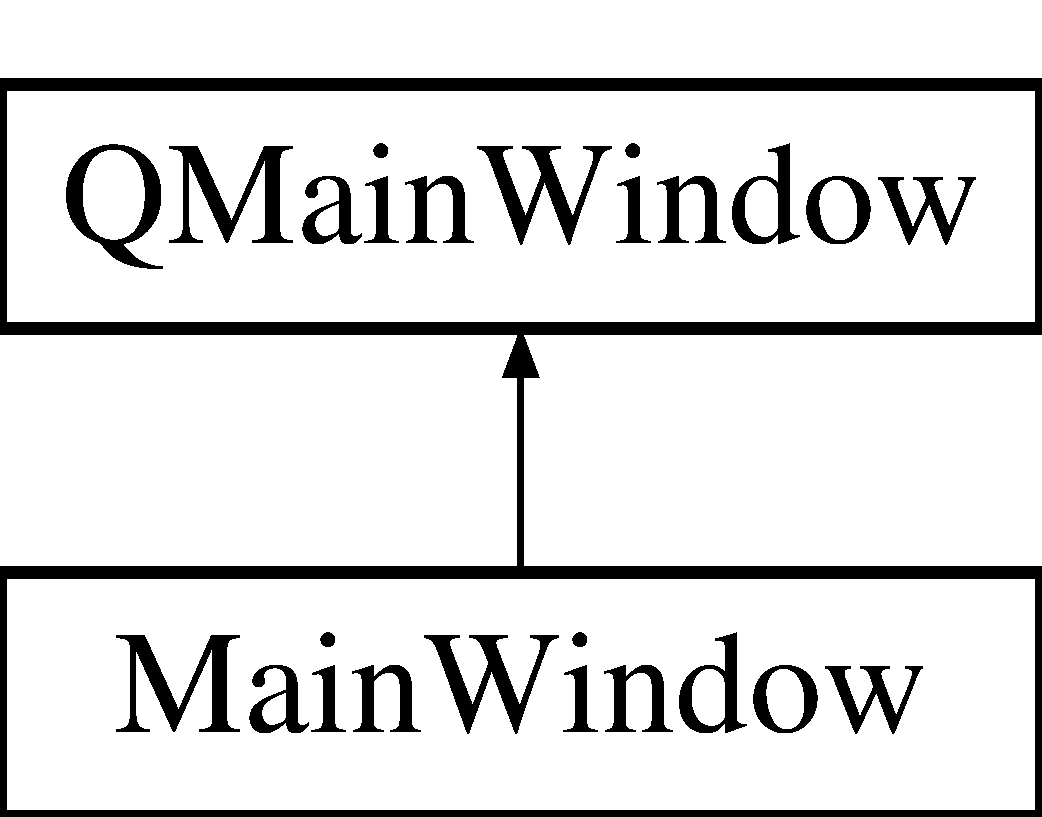
\includegraphics[height=2.000000cm]{classMainWindow}
\end{center}
\end{figure}
\subsection*{Public Member Functions}
\begin{DoxyCompactItemize}
\item 
\hypertarget{classMainWindow_a8b244be8b7b7db1b08de2a2acb9409db}{{\bfseries Main\-Window} (Q\-Widget $\ast$parent=0)}\label{classMainWindow_a8b244be8b7b7db1b08de2a2acb9409db}

\item 
\hypertarget{classMainWindow_a597a4a602b7ebad94f2eec86a0db7563}{void {\bfseries set\-Main\-Data} ()}\label{classMainWindow_a597a4a602b7ebad94f2eec86a0db7563}

\item 
\hypertarget{classMainWindow_a75ce441f08138eca2ef1665a66870a43}{void {\bfseries get\-Main\-Data} ()}\label{classMainWindow_a75ce441f08138eca2ef1665a66870a43}

\end{DoxyCompactItemize}
\subsection*{Static Public Attributes}
\begin{DoxyCompactItemize}
\item 
\hypertarget{classMainWindow_aa26df84f6e0c27464332427cec49d8a9}{static Q\-String {\bfseries T\-I\-T\-L\-E}}\label{classMainWindow_aa26df84f6e0c27464332427cec49d8a9}

\end{DoxyCompactItemize}


The documentation for this class was generated from the following file\-:\begin{DoxyCompactItemize}
\item 
/home/boris/dokumenty/\-S\-U\-R\-O/medipix/experiment/\-Rn/\-Progeny\-\_\-\-U\-I/src/mainwindow.\-h\end{DoxyCompactItemize}

\hypertarget{structMainWindowData}{\section{Main\-Window\-Data Struct Reference}
\label{structMainWindowData}\index{Main\-Window\-Data@{Main\-Window\-Data}}
}
\subsection*{Data Fields}
\begin{DoxyCompactItemize}
\item 
\hypertarget{structMainWindowData_a13e994aac6efee77384aadf76389582c}{string {\bfseries name}}\label{structMainWindowData_a13e994aac6efee77384aadf76389582c}

\item 
\hypertarget{structMainWindowData_a3a1ed9bff4936fc9560c58c9d7cee92b}{string {\bfseries db\-Name}}\label{structMainWindowData_a3a1ed9bff4936fc9560c58c9d7cee92b}

\item 
\hypertarget{structMainWindowData_a1ad60e01af91667077554f87680a3c85}{double {\bfseries lambda} \mbox{[}3\mbox{]}}\label{structMainWindowData_a1ad60e01af91667077554f87680a3c85}

\item 
\hypertarget{structMainWindowData_a3fbc2c6f48e91f8db2b6115398ef4dde}{double {\bfseries filt\-\_\-time}}\label{structMainWindowData_a3fbc2c6f48e91f8db2b6115398ef4dde}

\item 
\hypertarget{structMainWindowData_aed7b2a7e280cf3fd1ff1195034b6f085}{double {\bfseries eff\-\_\-filter}}\label{structMainWindowData_aed7b2a7e280cf3fd1ff1195034b6f085}

\item 
\hypertarget{structMainWindowData_ac3b16f98ddcb0bf66df80b8a9d3b60b5}{double {\bfseries volume}}\label{structMainWindowData_ac3b16f98ddcb0bf66df80b8a9d3b60b5}

\end{DoxyCompactItemize}


The documentation for this struct was generated from the following file\-:\begin{DoxyCompactItemize}
\item 
/home/boris/dokumenty/\-S\-U\-R\-O/medipix/experiment/\-Rn/\-Progeny\-\_\-\-U\-I/src/datahandle.\-h\end{DoxyCompactItemize}

\hypertarget{classProgenyMatrix}{\section{Progeny\+Matrix Class Reference}
\label{classProgenyMatrix}\index{Progeny\+Matrix@{Progeny\+Matrix}}
}
\subsection*{Public Member Functions}
\begin{DoxyCompactItemize}
\item 
\hypertarget{classProgenyMatrix_a79232328f0be2c397ea9773c44f4913a}{{\bfseries Progeny\+Matrix} (const double $\ast$lambda, const double T=0)}\label{classProgenyMatrix_a79232328f0be2c397ea9773c44f4913a}

\item 
\hypertarget{classProgenyMatrix_a5fef82dcd5a0ff2b430852c92d407817}{void {\bfseries set\+Coeficients} (const double $\ast$lambda, const double T=0)}\label{classProgenyMatrix_a5fef82dcd5a0ff2b430852c92d407817}

\item 
\hypertarget{classProgenyMatrix_a0563a137e4337096eaebddad9cc1179b}{vector$<$ double $>$ {\bfseries get\+Conc\+From\+Inf\+Alphas} (const double $\ast$par)}\label{classProgenyMatrix_a0563a137e4337096eaebddad9cc1179b}

\item 
\hypertarget{classProgenyMatrix_ac4221da6b1d4a1c829aac5774260d516}{vector$<$ double $>$ {\bfseries get\+Conc\+From\+Alphas} (const double $\ast$par, const double \&time\+Delta)}\label{classProgenyMatrix_ac4221da6b1d4a1c829aac5774260d516}

\item 
\hypertarget{classProgenyMatrix_a53752e6ed1f655caa2761e5416f00128}{double {\bfseries get\+Activity\+Filter} (const int \&which, const double $\ast$conc, const double \&a\+Time, const double \&volume\+Filtered, const double \&time\+Filtration)}\label{classProgenyMatrix_a53752e6ed1f655caa2761e5416f00128}

\item 
\hypertarget{classProgenyMatrix_adf1b00db95a9dd67932e441ac9370970}{double {\bfseries get\+Num\+Particles} (const int \&which, const double $\ast$conc, const double \&a\+Time, const double time\+Delta=0)}\label{classProgenyMatrix_adf1b00db95a9dd67932e441ac9370970}

\item 
\hypertarget{classProgenyMatrix_af828e1acd29997e9c7f4ade2606b0d18}{double {\bfseries get\+Num\+Particles} (const int \&which, const double $\ast$conc, const double \&a\+Time, const double time\+Delta, const double volume\+Filtered, double time\+Filtration=0)}\label{classProgenyMatrix_af828e1acd29997e9c7f4ade2606b0d18}

\item 
\hypertarget{classProgenyMatrix_adc511e5bb07ef655fb085b31232072b6}{vector$<$ double $>$ {\bfseries get\+Progeny\+Wihout\+Filter} (const double $\ast$N, const double t)}\label{classProgenyMatrix_adc511e5bb07ef655fb085b31232072b6}

\item 
\hypertarget{classProgenyMatrix_af7c7f969cd87add705bd2a6aa1bf323d}{vector$<$ double $>$ {\bfseries get\+Num\+Created\+Particles} (const double $\ast$N, const double t, const double time\+Delta)}\label{classProgenyMatrix_af7c7f969cd87add705bd2a6aa1bf323d}

\item 
\hypertarget{classProgenyMatrix_a9420c56c7afbb8950822da28ab7249c9}{vector$<$ double $>$ {\bfseries get\+Num\+Particles} (const double $\ast$N, const double time\+Delta)}\label{classProgenyMatrix_a9420c56c7afbb8950822da28ab7249c9}

\item 
\hypertarget{classProgenyMatrix_a610583b083ef3a46ff2471d4ab06412e}{void {\bfseries test} ()}\label{classProgenyMatrix_a610583b083ef3a46ff2471d4ab06412e}

\end{DoxyCompactItemize}
\subsection*{Friends}
\begin{DoxyCompactItemize}
\item 
\hypertarget{classProgenyMatrix_ab98de18a4e21a01349e72a4a5ebfef6d}{ostream \& {\bfseries operator$<$$<$} (ostream \&stream, const \hyperlink{classProgenyMatrix}{Progeny\+Matrix} \&progeny\+Matrix)}\label{classProgenyMatrix_ab98de18a4e21a01349e72a4a5ebfef6d}

\item 
\hypertarget{classProgenyMatrix_a849973a8862cb5f5343512e200fe2687}{ostream \& {\bfseries operator$<$$<$} (ostream \&stream, const \hyperlink{classProgenyMatrix}{Progeny\+Matrix} $\ast$progeny\+Matrix)}\label{classProgenyMatrix_a849973a8862cb5f5343512e200fe2687}

\end{DoxyCompactItemize}


The documentation for this class was generated from the following file\+:\begin{DoxyCompactItemize}
\item 
/home/boris/dokumenty/\+S\+U\+R\+O/medipix/programy/\+Progeny\+\_\+\+U\+I/src/progeny\+Matrix.\+hh\end{DoxyCompactItemize}

\hypertarget{classSqlConnection}{\section{Sql\+Connection Class Reference}
\label{classSqlConnection}\index{Sql\+Connection@{Sql\+Connection}}
}


Class for showing, selecting sql database. Class for insertion and obtaining data is \hyperlink{classSqlHandle}{Sql\+Handle}.  




{\ttfamily \#include $<$sqlconnection.\+h$>$}

Inheritance diagram for Sql\+Connection\+:\begin{figure}[H]
\begin{center}
\leavevmode
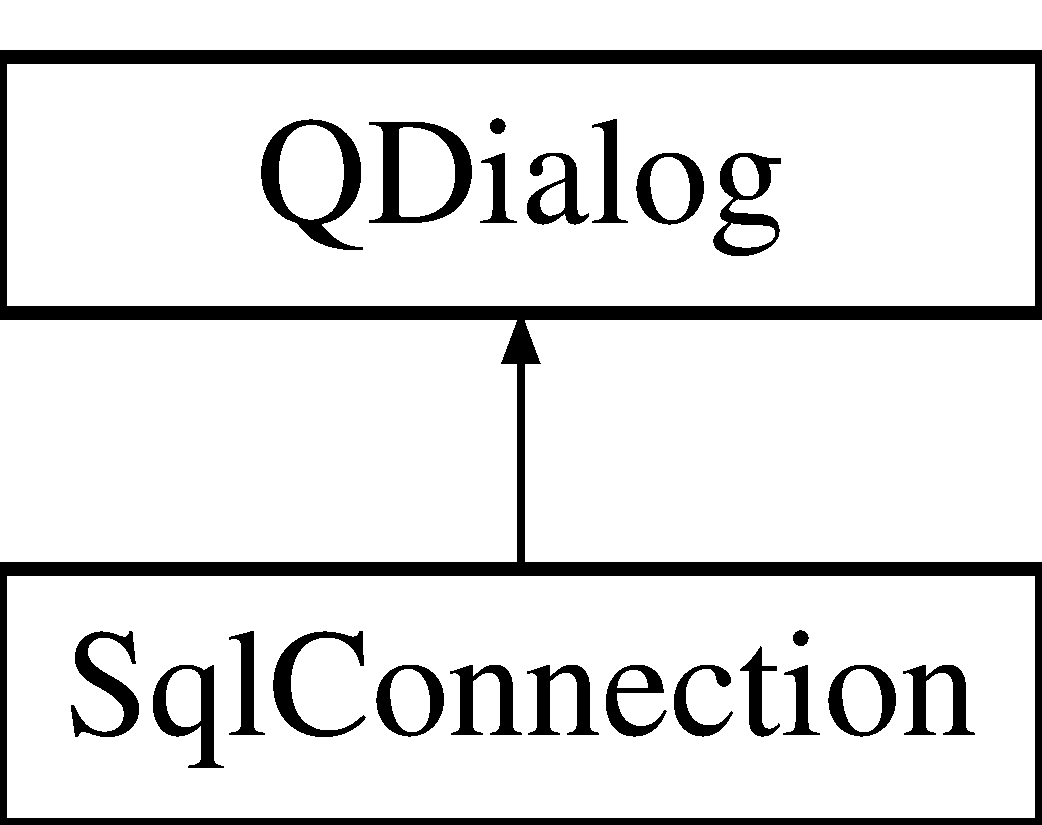
\includegraphics[height=2.000000cm]{classSqlConnection}
\end{center}
\end{figure}
\subsection*{Public Slots}
\begin{DoxyCompactItemize}
\item 
\hypertarget{classSqlConnection_a82e3b42ecea79904550546acbcef70b7}{void {\bfseries update\+Table\+From\+Command} ()}\label{classSqlConnection_a82e3b42ecea79904550546acbcef70b7}

\item 
\hypertarget{classSqlConnection_ade9e50f4c19e51e1229c2c71f0ae7be4}{void {\bfseries show\+Table} (const Q\+String \&t)}\label{classSqlConnection_ade9e50f4c19e51e1229c2c71f0ae7be4}

\item 
\hypertarget{classSqlConnection_a42fec1968d2a28aed8a130a3851715ee}{void {\bfseries on\+\_\+action\+Fetch\+Db\+\_\+triggered} ()}\label{classSqlConnection_a42fec1968d2a28aed8a130a3851715ee}

\item 
\hypertarget{classSqlConnection_a585556486aefb0e01764c299678a7998}{void {\bfseries on\+\_\+action\+Insert\+Row\+\_\+triggered} ()}\label{classSqlConnection_a585556486aefb0e01764c299678a7998}

\item 
\hypertarget{classSqlConnection_a54e2f239aa237f1eed5e4c6023c2001a}{void {\bfseries on\+\_\+action\+Delete\+Row\+\_\+triggered} ()}\label{classSqlConnection_a54e2f239aa237f1eed5e4c6023c2001a}

\item 
\hypertarget{classSqlConnection_ac11db1288aa22bee6a645f006665558e}{void {\bfseries current\+Changed} ()}\label{classSqlConnection_ac11db1288aa22bee6a645f006665558e}

\end{DoxyCompactItemize}
\subsection*{Signals}
\begin{DoxyCompactItemize}
\item 
\hypertarget{classSqlConnection_add3790e6a432367e0df8774d952a74da}{void {\bfseries status\+Message} (const Q\+String \&message)}\label{classSqlConnection_add3790e6a432367e0df8774d952a74da}

\end{DoxyCompactItemize}
\subsection*{Public Member Functions}
\begin{DoxyCompactItemize}
\item 
\hypertarget{classSqlConnection_ad936fc98369d3e3f0471aee180d8a80a}{{\bfseries Sql\+Connection} (Q\+Widget $\ast$parent=0)}\label{classSqlConnection_ad936fc98369d3e3f0471aee180d8a80a}

\item 
\hypertarget{classSqlConnection_a2f0318c01899357ce4a3092e2993f6d3}{bool {\bfseries is\+Open\+Db} ()}\label{classSqlConnection_a2f0318c01899357ce4a3092e2993f6d3}

\item 
\hypertarget{classSqlConnection_aa03f1185085e3f8607bcf1f607a60a22}{virtual void {\bfseries accept} ()}\label{classSqlConnection_aa03f1185085e3f8607bcf1f607a60a22}

\item 
\hypertarget{classSqlConnection_a9279e66a9187e4fc47b00b8883085352}{const Q\+Table\+View $\ast$ {\bfseries get\+Info1\+Table} () const }\label{classSqlConnection_a9279e66a9187e4fc47b00b8883085352}

\item 
\hypertarget{classSqlConnection_ac12be705fcd20869aeca038b5de97136}{int {\bfseries get\+Sql\+Entry} (const int I\+D)}\label{classSqlConnection_ac12be705fcd20869aeca038b5de97136}

\item 
\hypertarget{classSqlConnection_a12cb9b234c9c46517015232d3e712203}{void {\bfseries insert\+Row} ()}\label{classSqlConnection_a12cb9b234c9c46517015232d3e712203}

\item 
\hypertarget{classSqlConnection_a2f7155fdf28187d4328c28b0ead736e7}{void {\bfseries delete\+Row} ()}\label{classSqlConnection_a2f7155fdf28187d4328c28b0ead736e7}

\item 
\hypertarget{classSqlConnection_a1f632f61a1baa84358b04600fd5cf1c6}{void {\bfseries update\+Actions} ()}\label{classSqlConnection_a1f632f61a1baa84358b04600fd5cf1c6}

\item 
\hypertarget{classSqlConnection_aa6435ff7a964d00418457111f6f33380}{void {\bfseries show\+Db\+Table} ()}\label{classSqlConnection_aa6435ff7a964d00418457111f6f33380}

\item 
\hypertarget{classSqlConnection_ab497606fdbaefeedf5c9d4223fea3a1d}{void {\bfseries only\+For\+Save} ()}\label{classSqlConnection_ab497606fdbaefeedf5c9d4223fea3a1d}

\item 
\hypertarget{classSqlConnection_a859135cab392d805adc40a58f6d0adf9}{void {\bfseries only\+For\+Open} ()}\label{classSqlConnection_a859135cab392d805adc40a58f6d0adf9}

\end{DoxyCompactItemize}
\subsection*{Static Public Attributes}
\begin{DoxyCompactItemize}
\item 
\hypertarget{classSqlConnection_a0d53b0970637eed7f37c8190fdb2095a}{static bool {\bfseries I\+S\+\_\+\+S\+A\+V\+E}}\label{classSqlConnection_a0d53b0970637eed7f37c8190fdb2095a}

\end{DoxyCompactItemize}


\subsection{Detailed Description}
Class for showing, selecting sql database. Class for insertion and obtaining data is \hyperlink{classSqlHandle}{Sql\+Handle}. 

The documentation for this class was generated from the following file\+:\begin{DoxyCompactItemize}
\item 
/home/boris/dokumenty/\+S\+U\+R\+O/medipix/programy/\+Progeny\+\_\+\+U\+I/src/sqlconnection.\+h\end{DoxyCompactItemize}

\hypertarget{classSqlHandle}{\section{Sql\-Handle Class Reference}
\label{classSqlHandle}\index{Sql\-Handle@{Sql\-Handle}}
}
\subsection*{Public Member Functions}
\begin{DoxyCompactItemize}
\item 
\hypertarget{classSqlHandle_a74881baa2b268e2507d361007ca3d071}{void {\bfseries create\-Main\-Tables} ()}\label{classSqlHandle_a74881baa2b268e2507d361007ca3d071}

\item 
\hypertarget{classSqlHandle_a09cc807b1fb5aeda615ba8081f66cc1f}{void {\bfseries create\-Second\-Table} (const int I\-D)}\label{classSqlHandle_a09cc807b1fb5aeda615ba8081f66cc1f}

\item 
\hypertarget{classSqlHandle_a7a0d2c81551b031837bbea9cf97b513e}{void {\bfseries insert\-Into\-Main\-Info\-Table} (const \hyperlink{structMainWindowData}{Main\-Window\-Data} \&main\-Window\-Data)}\label{classSqlHandle_a7a0d2c81551b031837bbea9cf97b513e}

\item 
\hypertarget{classSqlHandle_ac111d82dcd20a975ab64563313403c5f}{void {\bfseries delete\-Measurement} (const int I\-D)}\label{classSqlHandle_ac111d82dcd20a975ab64563313403c5f}

\item 
\hypertarget{classSqlHandle_a8cbd20e9edad986197ceec01897442e7}{const vector$<$ Data $>$ {\bfseries get\-Sql\-Data} (const int I\-D)}\label{classSqlHandle_a8cbd20e9edad986197ceec01897442e7}

\item 
\hypertarget{classSqlHandle_a9e63022701c72474a6baf13f581fbc02}{Data {\bfseries get\-Data\-From\-Query} (const Q\-Sql\-Query \&query, const Q\-Sql\-Record \&record)}\label{classSqlHandle_a9e63022701c72474a6baf13f581fbc02}

\end{DoxyCompactItemize}
\subsection*{Static Public Member Functions}
\begin{DoxyCompactItemize}
\item 
\hypertarget{classSqlHandle_a508226e88c14ca5d276cc767f6572b71}{static \hyperlink{classSqlHandle}{Sql\-Handle} $\ast$ {\bfseries get\-Instance} ()}\label{classSqlHandle_a508226e88c14ca5d276cc767f6572b71}

\item 
\hypertarget{classSqlHandle_a15e01a13e792ddd03ecfe81f0b19b002}{static void {\bfseries insert\-Into\-Second\-Table} (const int I\-D, const int measurement)}\label{classSqlHandle_a15e01a13e792ddd03ecfe81f0b19b002}

\item 
\hypertarget{classSqlHandle_ada1895a0832932054445a2548a44b5f8}{static void {\bfseries insert\-Into\-Third\-Table} (const int I\-D, const int measurement)}\label{classSqlHandle_ada1895a0832932054445a2548a44b5f8}

\end{DoxyCompactItemize}


The documentation for this class was generated from the following file\-:\begin{DoxyCompactItemize}
\item 
/home/boris/dokumenty/\-S\-U\-R\-O/medipix/experiment/\-Rn/\-Progeny\-\_\-\-U\-I/src/sqlhandle.\-h\end{DoxyCompactItemize}

\input{structTimeDependenceWindowData}
%--- End generated contents ---

% Index
\newpage
\phantomsection
\addcontentsline{toc}{chapter}{Index}
\printindex

\end{document}
